%%%%%%%%%%%%%%%%%%%%%%%%%%%%%%%%%%
% EL/EEE D1 Report Template
% University of Southampton
%
% author : Rhys Thomas (rt8g15)
%
% edited : 2016-11-14
%%%%%%%%%%%%%%%%%%%%%%%%%%%%%%%%%%

\documentclass[a4paper,11pt]{article}

%%%%%%%%%%%%%%%%%%%%%%%%%%%%%%%%%%
% PACKAGES
%%%%%%%%%%%%%%%%%%%%%%%%%%%%%%%%%%
\usepackage[margin=1in]{geometry}
\renewcommand{\baselinestretch}{1.2} % line spacing
\usepackage{color}
\usepackage{siunitx}
\usepackage{graphicx}
\usepackage{epstopdf}
\usepackage{float}
\usepackage{pdfpages}
\usepackage{hyperref}
\usepackage{mathtools}
\usepackage{csvsimple}
\usepackage[titletoc,toc,title]{appendix}
\usepackage{pgfplots}
\usepackage{subfiles}
\usepackage{subfig}

\pgfplotsset{compat=1.13}

\graphicspath{ {./images/} }

%%%%%%%%%%%%%%%%%%%%%%%%%%%%%%%%%%
% DOCUMENT BEGIN
%%%%%%%%%%%%%%%%%%%%%%%%%%%%%%%%%%
\begin{document}
  
\begin{center}
{\Large{\textbf{ELEC2201 P1 -- Solar cell research exercise}}} \\ [\baselineskip]
\subfile{info.tex}
\end{center}

\begin{abstract}
I really hope I don't forget to go back to this at the end...
\end{abstract}

\section{Aim}
The aim of this set of experiments was to measure and analyse the Current-Voltage characteristics of a solar cell, as well as its performance, and how it varies in different conditions that may arise in the real world.

The experimental setup included a tungsten lamp pointed at single solar cell, which is mounted on to a peltier cooler/heater.

\section{Hypothesis}
Three experiments were carried out to measure the IV characteristics of the solar cell. The first involved varying the series resistance of the cell from \SI{1}{\ohm}, to \SI{9999}{\ohm}. The expected result was that as the resistance increased, the voltage across the resistance would increase, and therefore the current would decrease following a typical solar cell IV curve, such as the one shown in figure \ref{fig:moduleIV}.

\begin{figure}[h]
    \centering
    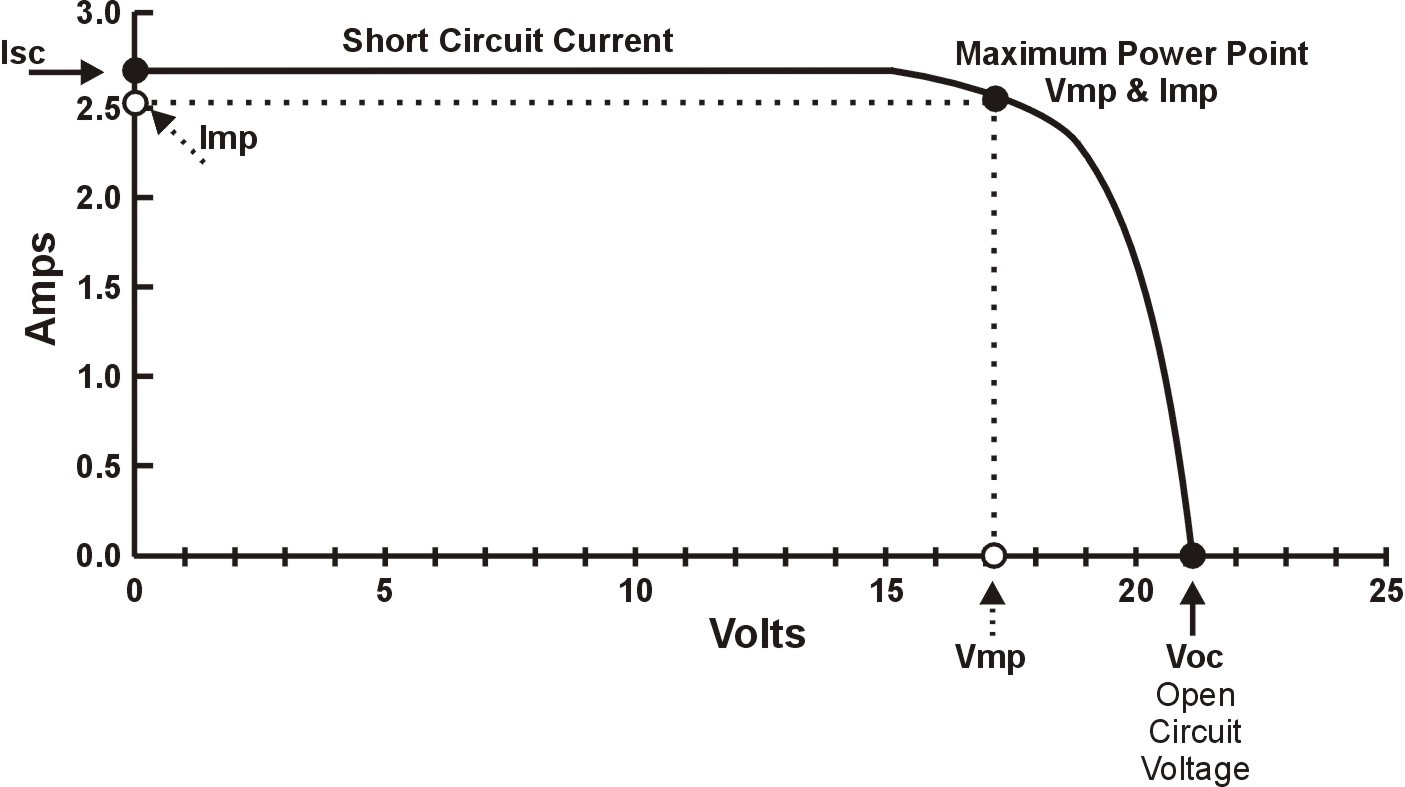
\includegraphics{moduleIV.jpg}
    \caption{An example of an IV characteristic graph for a solar cell~\cite{moduleIV}.}
    \label{fig:moduleIV}
\end{figure}

The second experiment measured the output voltage of the solar cell at varying light intensities and series resistances. It was hypothesised that an increase in light intensity would increase the voltage across the cell. The intensity was varied by adjusting the distance between the light source and the cell.

The third experiment measured the output voltage of the solar cell at varying temperatures. The hypothesis was that as the temperature of the cell was increased, its output voltage would decrease, as shown by equation~\ref{eq:V_OC}. Increasing the temperature, $T$, would decrease the bandgap energy of the semiconductor, and the intrinsic carrier concentration, $n_i$, which would increase the saturation current, $I_0$, decreasing the open circuit voltage, $V_{OC}$.

\begin{equation} \label{eq:V_OC}
V_{OC} = \frac{nkT}{q}\ln{\left(\frac{I_L}{I_0} + 1\right)}
\end{equation}


\section{Results}
\subsection{Baseline data}

This was the simple experiment that involved measuring the voltage across a varying resistance. The light source was fixed at \SI{10}{\centi\metre}, and the cell was kept at a temperature of \SI{25}{\celsius}.

\begin{figure}[h]
\begin{tikzpicture}
    \begin{axis}[
        width = \textwidth,
        height = 0.4\textheight,
        xlabel = {Voltage},
        ylabel = {Current},
        grid = both
        ]
        \addplot table[x = Voltage, y = Current, col sep = comma]{./tables/baseline.csv};
    \end{axis}
\end{tikzpicture}
\label{plot:baseline}
\caption{Scatter plot for the acquired baseline data, based on the data from Appendix~\ref{dat:baseline}}
\end{figure}

\subsection{Varying light intensity}

The above experiment was repeated, but at various light intensities. The intensity was varied by adjusting the distance between the light source and the solar cell.

\begin{figure}[H]
\centering
    \subfloat[Subfigure 1 list of figures text][Light \SI{20}{\centi\metre} from cell (Appendix~\ref{dat:d20}).]{
        \begin{tikzpicture}
            \begin{axis}[
                width = 0.5\textwidth,
                height = 0.3\textheight,
                xlabel = {Voltage},
                ylabel = {Current},
                grid = both
                ]
                \addplot table[x = Voltage, y = Current, col sep = comma]{./tables/distance20.csv};
            \end{axis}
        \end{tikzpicture}
        \label{plot:d20}
    }
    \subfloat[Subfigure 1 list of figures text][Light \SI{30}{\centi\metre} from cell (Appendix~\ref{dat:d30}).]{
        \begin{tikzpicture}
            \begin{axis}[
                width = 0.5\textwidth,
                height = 0.3\textheight,
                xlabel = {Voltage},
                ylabel = {Current},
                grid = both
                ]
                \addplot table[x = Voltage, y = Current, col sep = comma]{./tables/distance30.csv};
            \end{axis}
        \end{tikzpicture}
        \label{plot:d30}
    }
    \qquad
    \subfloat[Subfigure 1 list of figures text][Light \SI{40}{\centi\metre} from cell (Appendix~\ref{dat:d40}).]{
        \begin{tikzpicture}
            \begin{axis}[
                width = 0.5\textwidth,
                height = 0.3\textheight,
                xlabel = {Voltage},
                ylabel = {Current},
                grid = both
                ]
                \addplot table[x = Voltage, y = Current, col sep = comma]{./tables/distance40.csv};
            \end{axis}
        \end{tikzpicture}
        \label{plot:d40}
    }
    \subfloat[Subfigure 1 list of figures text][Light \SI{50}{\centi\metre} from cell (Appendix~\ref{dat:d50}).]{
        \begin{tikzpicture}
            \begin{axis}[
                width = 0.5\textwidth,
                height = 0.3\textheight,
                xlabel = {Voltage},
                ylabel = {Current},
                grid = both
                ]
                \addplot table[x = Voltage, y = Current, col sep = comma]{./tables/distance50.csv};
            \end{axis}
        \end{tikzpicture}
        \label{plot:d50}
    }
    \caption{Scatter plots for varying light intensity.}
    \label{fig:globfig}
\end{figure}

\section{Analysis}


\section{Conclusion}


\section{Evaluation}


\begin{appendices}
    \label{appendix}
    \section{Baseline data}
    \label{dat:baseline}
        \csvautotabular{./tables/baseline.csv}
    
    \section{Varying light intensity - \SI{20}{\centi\metre}}
    \label{dat:d20}
        \csvautotabular{./tables/distance20.csv}
        
    \section{Varying light intensity - \SI{30}{\centi\metre}}
    \label{dat:d30}
        \csvautotabular{./tables/distance30.csv}
        
    \section{Varying light intensity - \SI{40}{\centi\metre}}
    \label{dat:d40}
        \csvautotabular{./tables/distance40.csv}
        
    \section{Varying light intensity - \SI{50}{\centi\metre}}
    \label{dat:d50}
        \csvautotabular{./tables/distance50.csv}
\end{appendices}

\bibliographystyle{IEEEtran}
% IEEEabrv abbreviates journal titles in accordance to IEEE standards 
\bibliography{mybib}

\end{document}